\documentclass[12pt]{article} 
\usepackage{longtable}
\usepackage{makecell}
\usepackage{float}
\usepackage{graphicx}
\usepackage{bm}
\usepackage{placeins}
\usepackage{booktabs}
\usepackage{gensymb}
\usepackage{subcaption}
\usepackage{amssymb}
\usepackage{indentfirst}
\usepackage{threeparttable} 
\usepackage{multirow}
\usepackage{tabularx}
\usepackage{aligned-overset}
\usepackage[slantfont,boldfont]{xeCJK}
\usepackage{fontspec}
\renewcommand{\arraystretch}{1.5}
% \usepackage[paperwidth=21cm,paperheight=29.7cm]{geometry}
\usepackage[a4paper,margin=2cm]{geometry}
\setCJKmainfont{SimSun}
\setmainfont{SimSun}
\setsansfont{SimSun}
% 设置正文字体为四号（12pt）
% \renewcommand{\CJKmainfont}{SimSun}
\renewcommand{\CJKfamilydefault}{\CJKrmdefault}
\renewcommand{\normalsize}{\fontsize{12pt}{18pt}\selectfont}
\normalsize

\title{交流电桥实验报告}
\author{2411545 邱凯锐}
\date{2025.12.19}

\begin{document}
\maketitle
\section{目的要求}
1. 掌握交流电桥的平衡条件和测量原理；

2. 掌握交流电桥平衡的调节方法；

\section{实验原理}

\subsection{电感、电容元件的等效电路及有关参数}

\subsubsection{电感}

一个实际的电感线圈可以等效为一个理想的纯电感 $L$ 和直流损耗电阻 $r$ 串联而成。用品质因数 $Q$ 来标志电感元件品质的好坏。其定义为电感线圈的无功功率 $P_{无功}$ 和有功功率 $P_{有功}$ 之比。对于 $L$ 和 $r$ 串联等效的电感来说，有
\begin{equation}
    Q=\frac{P_{无功}}{P_{有功}}=\frac{\omega L}{r}
\end{equation}
$Q$ 越高表示 $P_{有功}$ （即各种损耗）越小，表明电感线圈的质量越佳。

\begin{figure}[H]
    \centering
    \begin{subfigure}[c]{0.3\textwidth}
        \centering
        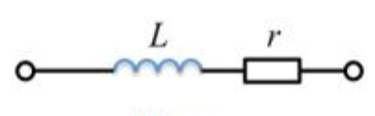
\includegraphics[width=\textwidth]{fig1a.png}
    \end{subfigure}
    \hfil
    \begin{subfigure}[c]{0.2\textwidth}
        \centering
        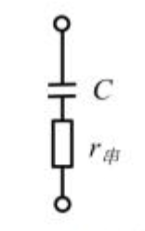
\includegraphics[width=\textwidth]{fig1b.png}
    \end{subfigure}
    \hfil
    \begin{subfigure}[c]{0.2\textwidth}
        \centering
        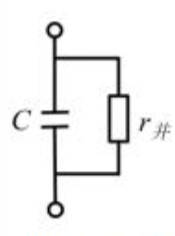
\includegraphics[width=\textwidth]{fig1c.png}
    \end{subfigure}
    \caption{}
\end{figure}


\subsubsection{电容}
实际的电容器常可用一个理想电容器和与之串联或并联的损耗电阻来等效。由于实际的电容器有介质损耗，所以正弦交流电通过它时，电容两端电压与通过它的电流之间的相位差 $\varphi$ 不是 $90^\circ$，而是 $\varphi=90^\circ-\delta$ 。角 $\delta$ 称为电容器的损耗角，显然 $\delta$ 角越小，实际的电容器和理想的电容器月接近。
常用损耗角 $\delta$ 的正切 $\mathrm{tg} \delta$ 来标志电容器的质量，并称为损耗因数。串、并联相对应的损耗因素分别为
\begin{equation}
    \mathrm{tg}\delta=
    \begin{cases}
        \omega Cr_{串}\\
        \dfrac{1}{\omega Cr_{并}}
    \end{cases}
\end{equation}

\subsection{交流电桥}
交流电桥的平衡条件为
\begin{equation}
    \boldsymbol{Z_1}\boldsymbol{Z_4}=\boldsymbol{Z_2}\boldsymbol{Z_3}
\end{equation}

\begin{figure}[H]
    \centering
    \begin{subfigure}[b]{0.3\textwidth}
        \centering
        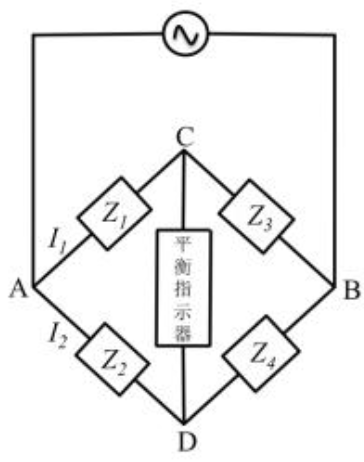
\includegraphics[width=\textwidth]{fig2a.png}
        \caption{交流电桥}
    \end{subfigure}
    \hfil
    \begin{subfigure}[b]{0.3\textwidth}
        \centering
        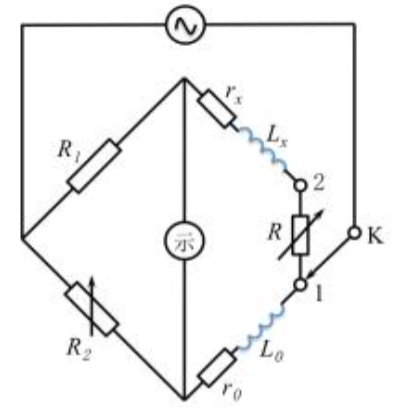
\includegraphics[width=\textwidth]{fig2b.png}
        \caption{电感电桥}
    \end{subfigure}
    \hfil
    \begin{subfigure}[b]{0.3\textwidth}
        \centering
        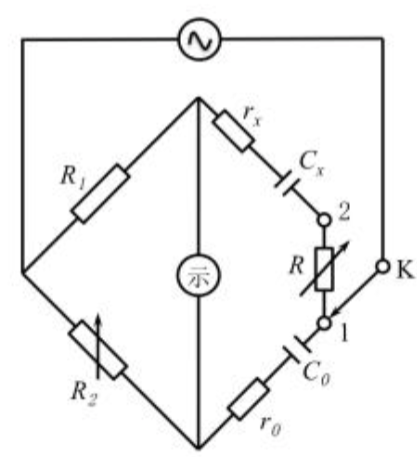
\includegraphics[width=\textwidth]{fig2c.png}
        \caption{电容电桥}
    \end{subfigure}
    \caption{}
\end{figure}

\subsubsection{电感电桥}
电感电桥的平衡条件
\begin{equation}
    \frac{R_1}{R_2}=\frac{L_x}{L_o}=\frac{r_x+R}{r_o}\quad K\ 置于“1”端
\end{equation}
\begin{equation}
    \frac{R_1}{R_2}=\frac{L_x}{L_o}=\frac{r_x}{r_o+R}\quad K\ 置于"2"端
\end{equation}
其中，$L_x$ 和 $r_x$ 为待测电感线圈的电感量和损耗电阻；$L_o$ 和 $r_o$ 为已知标准电感的电感量和损耗电阻；$R_1$、$R_2$ 为无感电阻，$R$ 为补偿电阻。
由式(4)和(5)可得 $L_x$ 和 $r_x$ 测量公式
\begin{equation}
    L_x=\frac{R_1}{R_2}L_o
\end{equation}
\begin{equation}
    r_x=\frac{R_1}{R_2}r_o-R\quad K\ 置于“1”端
\end{equation}
\begin{equation}
    r_x=\frac{R_1}{R_2}(r_o+R)\quad K\ 置于“2”端
\end{equation}

\subsubsection{电容电桥}
电容电桥的平衡条件为
\begin{equation}
    \frac{R_1}{R_2}=\frac{C_o}{C_x}=\frac{r_x+R}{r_o}\quad K\ 置于“1”端
\end{equation}
\begin{equation}
    \frac{R_1}{R_2}=\frac{C_o}{C_x}=\frac{r_x}{r_o+R}\quad K\ 置于“2”端
\end{equation}
其中，$C_x$ 和 $r_x$ 为待测电容器的电容和损耗电阻；$C_o$ 和 $r_o$ 为已知标准电容的电容量和损耗电阻；$R_1$、$R_2$ 为无感电阻，$R$ 为补偿电阻。
$C_x$ 和 $r_x$ 的测量公式
\begin{equation}
    C_x=\frac{R_2}{R_1}C_o
\end{equation}
\begin{equation}
    r_x=\frac{R_1}{R_2}r_o-R\quad K\ 置于“1”端
\end{equation}
\begin{equation}
    r_x=\frac{R_1}{R_2}(r_o+R)\quad K\ 置于“2”端
\end{equation}

\section{实验内容}
\subsection{实验仪器}
无感电阻箱 3 个，标准电感(0.1 H)一个，标准电容一个(0.1 $\mathrm \mu$F)，
信号发生器一台，示波器，待测电感，待测电容，导线若干。

\begin{figure}[H]
    \centering
    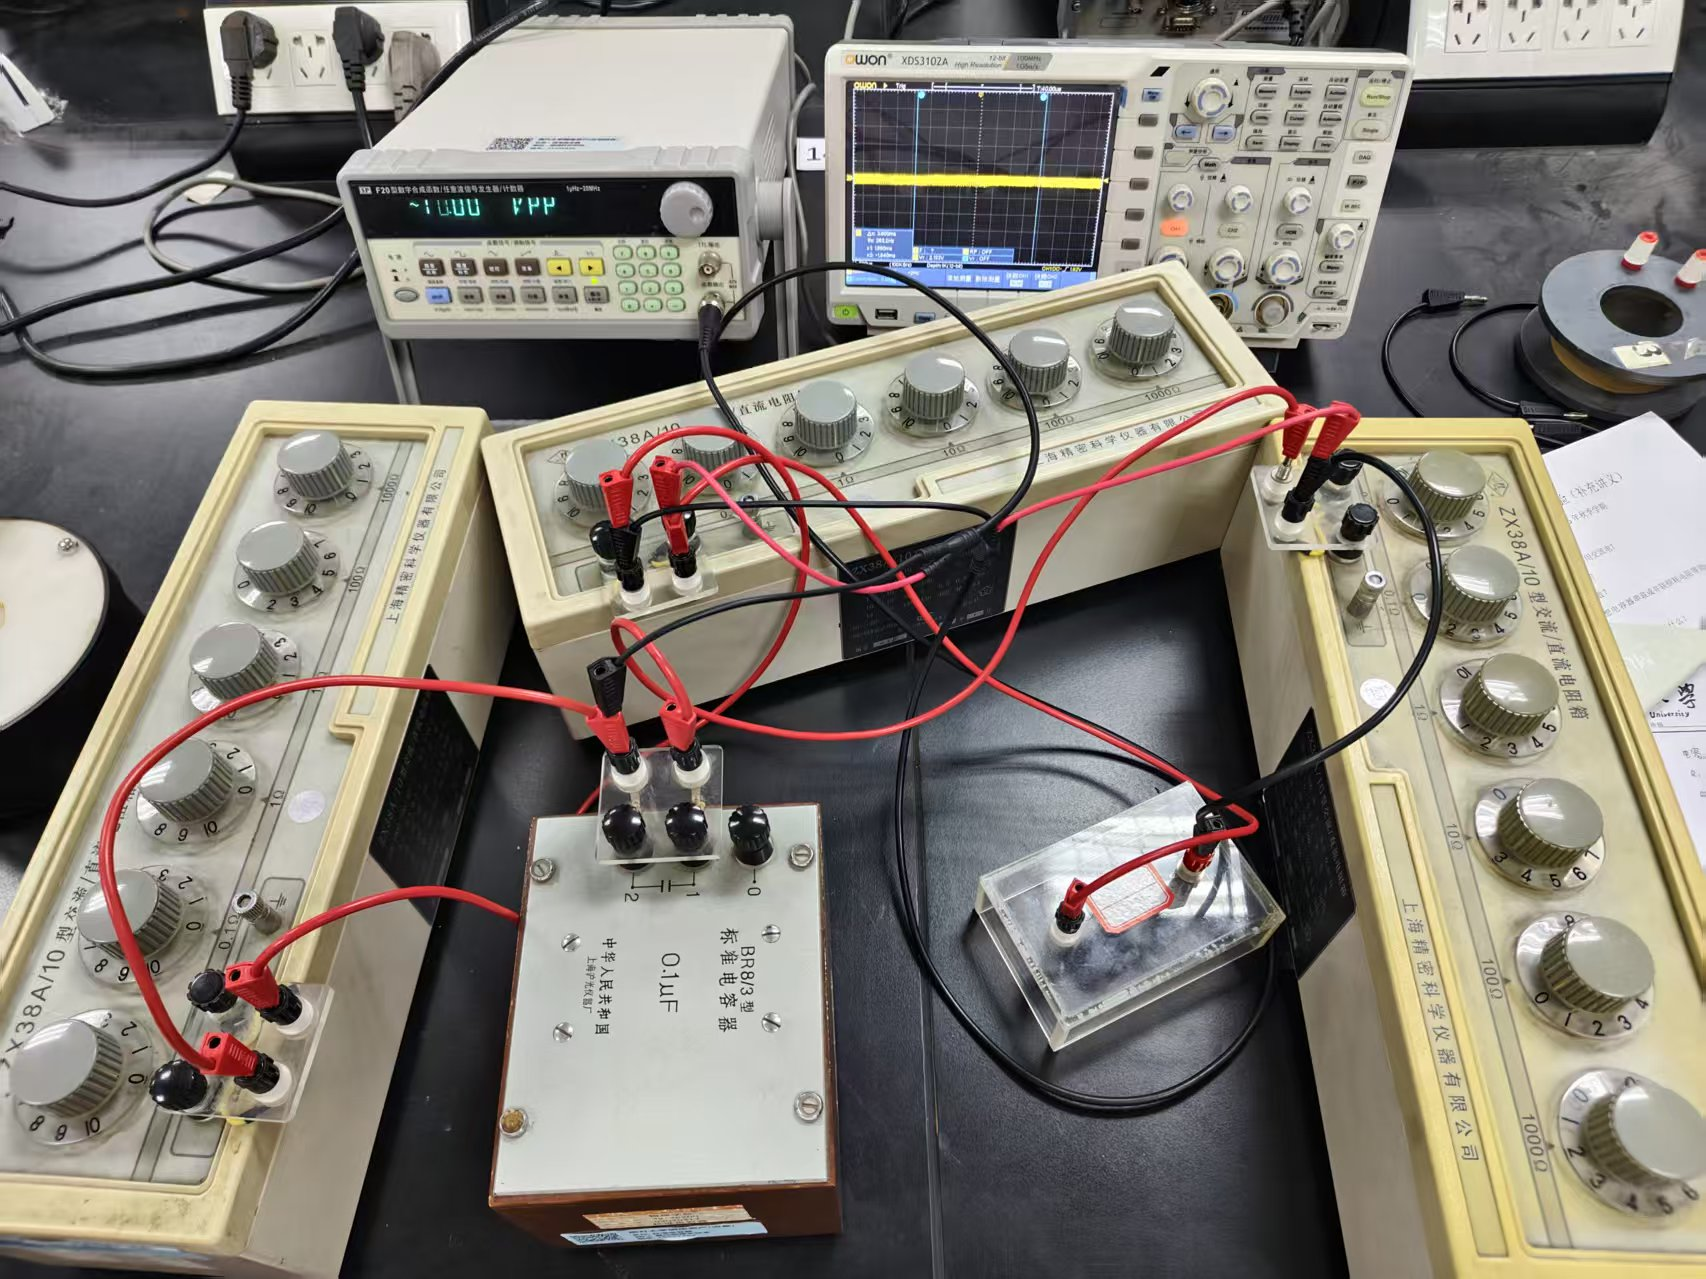
\includegraphics[width=0.4\textwidth]{fig4.jpg}
    \caption{}
\end{figure}

\subsection{电感器测量}
(1) 按照 Figure 2(b) 联接电路。信号发生器频率为 $1000Hz$，幅值为 $10V$。 $R_1$ 置于 $1000\Omega$ ，$R_2$ 和 $R$ 置零。

(2) 逐步调节 $R_2$ 的电阻值，使得示波器测量的电压值位于极小值。

(3) 先将 K 置于“1”端，若增大 $R$ 时，示波器的电压值增大，则将 K 置于“2”端。逐步调节 $R$ 的电阻值，使得示波器测量的电压值接近 0。记录此时 $R_2$，$R$ 的值。

\subsection{电容器测量}

(1) 按照 Figure 2(c) 联接电路。信号发生器频率为 $1000Hz$，幅值为 $10V$。 $R_1$ 置于 $1000\Omega$ ，$R_2$ 和 $R$ 置零。

(2) 逐步调节 $R_2$ 的电阻值，使得示波器测量的电压值位于极小值。

(3) 先将 K 置于“1”端，若增大 $R$ 时，示波器的电压值增大，则将 K 置于“2”端。逐步调节 $R$ 的电阻值，使得示波器测量的电压值接近 0。记录此时 $R_2$，$R$ 的值。


\section{实验数据}
\subsection{电感器测量}
\begin{table}[H]
    \centering
    \caption{电感器测量数据}
    \begin{minipage}{0.7\textwidth}
        \raggedleft
        K 置于“2”端，$f=1000Hz$
    \end{minipage}
    \begin{tabular}{ccccc}
        \hline\hline
        $R_1/\Omega$  & $R_2/\Omega$     & $R/\Omega$     & $L_o/H$ & $r_o/\Omega$   \\ \hline
        1000& 800 & 42 & 0.1 & 18.286 \\\hline\hline
       
    \end{tabular}
\end{table}
代入公式计算
\begin{equation}
    L_x=\frac{R_1}{R_2}L_o=0.125 H
\end{equation}
\begin{equation}
    r_x=\frac{R_1}{R_2}(r_o+R)=75,3575\Omega
\end{equation}
\begin{equation}
    Q=\frac{\omega L_x}{r_x}=10.42
\end{equation}
标准值为 $L_{标准}=0.12328 H$，$r_{标准}=64.349\Omega$，相对误差为
\begin{equation}
    E_{L}=\left|\dfrac{L_x-L_{标准}}{L_{标准}} \right|\times 100\%=1.40\%
\end{equation}
\begin{equation}
    E_{r}=\left|\dfrac{r_x-r_{标准}}{r_{标准}} \right|\times 100\%=17.11\%
\end{equation}

\subsection{电容器测量}
\begin{table}[H]
    \centering
    \caption{电容器测量数据}
    \begin{minipage}{0.7\textwidth}
        \raggedleft
        K 置于“2”端，$f=1000Hz$
    \end{minipage}
    \begin{tabular}{ccccc}
        \hline\hline
        $R_1/\Omega$  & $R_2/\Omega$     & $R/\Omega$     & $C_o/\mu F$ & $r_o/\Omega$   \\ \hline
        1000& 1510 & 15 & 0.1 & 0.29523 \\\hline\hline
       
    \end{tabular}
\end{table}
代入公式计算
\begin{equation}
    C_x=\frac{R_2}{R_1}C_o=0.151\mu F
\end{equation}
\begin{equation}
    r_x=\frac{R_2}{R_1}(r_o+R)=10.13\Omega
\end{equation}
\begin{equation}
    \mathrm{tg}\delta={\omega C_xr_x}=0.0096
\end{equation}
标准值为 $C_{标准}=0.15135\mu F$，$r_{标准}=8\Omega$，相对误差为
\begin{equation}
    E_C=\left|\frac{C_x-C_{标准}}{C_{标准}} \right|\times 100\%=0.23\%
\end{equation}
\begin{equation}
    E_r=\left|\frac{r_x-r_{标准}}{r_{标准}}\right|\times 100\%=26.62\%
\end{equation}

\subsection{误差分析}
(1) 由于噪声的存在，不可能将示波器的电压值完全调为零，即电桥并未完全平衡，使得测量值与理论值存在误差。

(2) 接线接头接触不良引起桥臂阻抗变化。

(3) 标准电感存在分布电容，简单等效为理向电感和损耗电阻串联造成了理论上的误差。

(4) 信号发生器产生的正弦波频率并不稳定，导致电感、电容的阻抗发生变化。

(5) 标准电感和电容老化，标注电感、电容值与实际有所出入。

\section{思考题}

(1) 根据你的实验结果，在电容电桥实验中，如果固定电阻 $R_1$ 变为 $1.8k\Omega$，理论计算出此时可变电阻 $R_2$,应当为多少(保留三位有效数字)?

\begin{equation}
    R_2=\frac{L_o}{L_x}R_1=1.44k\Omega
\end{equation}

(2) 根据你的实验结果，在电感电桥实验中，如果固定电阻 $R_1$ 变为 $1.8k\Omega$，此时可变电阻 $R_2$ 又是多少呢(保留三位有效数字)?
\begin{equation}
    R_2=\frac{C_x}{C_o}R_1=2.72k\Omega
\end{equation}


\end{document}